% answers.tex —— 2007 年·普通高等学校招生考试·山东卷·文科 · 参考答案与详细解析片段
% 由 tools/generate_projects.py 依来源总账自 2007/2007_数学真题_山东文_试题.md + 2007/2007_数学真题_山东文_解析正文.md + 2007/2007_数学真题_山东文_答案要点.md 生成，勿手改（改源 MD 后重跑）


\begin{gktip}
固定候选 PDF 仅含题面，无答案、解析和评分标准，原卷亦未标注分值；以下为非官方编者独立推导，官方答案字段为空。来源发布者、出版者、版次与官方身份均未核。
\end{gktip}

\begin{answer}
\gksolhead{1}{}

\textbf{题目}：

复数 $\dfrac{4+3\mathrm i}{1+2\mathrm i}$ 的实部是（　）

（A）$-2$

（B）$2$

（C）$3$

（D）$4$

\Needspace{4\baselineskip}
\textbf{解析}

\Needspace{5\baselineskip}
分子分母同乘 $1-2\mathrm i$：

\nopagebreak[4]
\[\frac{4+3\mathrm i}{1+2\mathrm i}=\frac{(4+3\mathrm i)(1-2\mathrm i)}{(1+2\mathrm i)(1-2\mathrm i)}=\frac{4-8\mathrm i+3\mathrm i-6\mathrm i^2}{1+4}=\frac{10-5\mathrm i}{5}=2-\mathrm i.\]

实部为 $2$，故选 B。

（判断要点：分母实数化时分子要完整乘 $1-2\mathrm i$；$\mathrm i^2=-1$，故 $3\mathrm i\cdot(-2\mathrm i)=+6$，不要算成 $-6$。）

\gkanswer{答案：B。}

\end{answer}
\begin{answer}
\gksolhead{2}{}

\textbf{题目}：

已知集合 $M=\{-1,1\}$，$N=\left\{x\;\middle|\;\dfrac12<2^{x+1}<4,\ x\in\mathbf Z\right\}$，则 $M\cap N=$（　）

（A）$\{-1,1\}$

（B）$\{-1\}$

（C）$\{0\}$

（D）$\{-1,0\}$

\Needspace{4\baselineskip}
\textbf{解析}

\Needspace{5\baselineskip}
由 $\dfrac12=2^{-1}$、$4=2^2$ 得

\nopagebreak[4]
\[2^{-1}<2^{x+1}<2^2,\]

\Needspace{5\baselineskip}
底数 $2>1$，故 $-1<x+1<2$，即 $-2<x<1$。又 $x\in\mathbf Z$，所以 $N=\{-1,0\}$，于是

\nopagebreak[4]
\[M\cap N=\{-1,1\}\cap\{-1,0\}=\{-1\},\]

选 B。

（判断要点：区间 $(-2,1)$ 内的整数是 $-1$ 与 $0$，两端点 $-2$、$1$ 都不取。）

\gkanswer{答案：B。}

\end{answer}
\begin{answer}
\gksolhead{3}{}

\textbf{题目}：

下列几何体各自的三视图中，有且仅有两个视图相同的是（　）
\nopagebreak[4]
\begin{center}% 2007 年山东卷文科第 3 题：四个几何体的直观图，自左至右为
%   ①正方体 ②圆锥 ③三棱台 ④正四棱锥，题问“各自的三视图中仅有两个相同”的是哪几个。
% 来源 PDF：gaokaomath-src/普通高考/2007/2007山东文.pdf
% SHA-256：64b760b73b0a8988bc87dd5d37fc646a10e257f357faf9ad7b1a17fdebaf4af3
% 原页：2007山东文.pdf 第 1 页（A3 三栏）第 1 栏，书页码 399，图在第 3 题题干下方。
% 重绘依据：按原页四个立体图形的位置与比例重绘，正方体、棱台、棱锥用斜投影，
%   圆锥底面用椭圆；被遮棱画虚线。下方标注①②③④及几何体名称。
\begin{tikzpicture}[scale=0.92, semithick,
  every node/.style={inner sep=1.5pt}]

  % ① 正方体
  \begin{scope}[shift={(0,0)}]
    \coordinate (A) at (0,0.35);
    \coordinate (B) at (1.25,0.35);
    \coordinate (C) at (1.25,1.60);
    \coordinate (D) at (0,1.60);
    \coordinate (A2) at (0.40,0.75);
    \coordinate (B2) at (1.65,0.75);
    \coordinate (C2) at (1.65,2.00);
    \coordinate (D2) at (0.40,2.00);
    \draw[dashed] (A2) -- (A);
    \draw[dashed] (A2) -- (B2);
    \draw[dashed] (A2) -- (D2);
    \draw (A) -- (B) -- (C) -- (D) -- cycle;
    \draw (A) -- (A2) -- (D2) -- (D);
    \draw (D2) -- (C2) -- (B2);
    \draw (C2) -- (C);
    \draw (B2) -- (B);
    \node[below] at (0.82,-0.12) {① 正方体};
  \end{scope}

  % ② 圆锥
  \begin{scope}[shift={(3.3,0.35)}]
    \draw (0,0) ellipse (0.78 and 0.22);
    \draw[dashed] (-0.78,0) arc (180:360:0.78 and 0.22);
    \draw (-0.78,0) -- (0,1.75) -- (0.78,0);
    \draw[dashed] (0,0) -- (0,1.75);
    \fill (0,0) circle (0.02);
    \node[below] at (0.02,-0.40) {② 圆锥};
  \end{scope}

  % ③ 三棱台
  \begin{scope}[shift={(6.3,0.0)}]
    \coordinate (P) at (0,0);
    \coordinate (Q) at (1.60,0);
    \coordinate (R) at (0.80,0.55);
    \coordinate (P1) at (0.28,1.30);
    \coordinate (Q1) at (1.28,1.30);
    \coordinate (R1) at (0.78,1.64);
    \draw[dashed] (P) -- (R);
    \draw[dashed] (R) -- (Q);
    \draw[dashed] (R) -- (R1);
    \draw (P) -- (Q);
    \draw (P) -- (P1);
    \draw (Q) -- (Q1);
    \draw (P1) -- (Q1) -- (R1) -- cycle;
    \draw (P1) -- (R1);
    \draw (Q1) -- (R1);
    \node[below] at (0.80,-0.12) {③ 三棱台};
  \end{scope}

  % ④ 正四棱锥
  \begin{scope}[shift={(9.6,0.0)}]
    \coordinate (A) at (0,0.35);
    \coordinate (B) at (1.35,0.35);
    \coordinate (C) at (1.75,0.85);
    \coordinate (D) at (0.40,0.85);
    \coordinate (S) at (0.88,2.05);
    \draw[dashed] (A) -- (D);
    \draw[dashed] (D) -- (C);
    \draw[dashed] (S) -- (D);
    \draw (A) -- (B) -- (C);
    \draw (S) -- (A);
    \draw (S) -- (B);
    \draw (S) -- (C);
    \node[below] at (0.85,0.02) {④ 正四棱锥};
  \end{scope}

\end{tikzpicture}
\end{center}
\nopagebreak[4]
（A）①②

（B）①③

（C）①④

（D）②④

\Needspace{4\baselineskip}
\textbf{解析}

逐个体判断。

① 正方体：三个视图都是全等正方形，不符合“仅有两个”。

② 圆锥：正视图与侧视图是全等等腰三角形，俯视图是带圆心的圆，恰有两个相同。

③ 三棱台：正视图与侧视图的梯形倾斜方向不同，俯视图是嵌套三角形，三个视图互不相同。

④ 正四棱锥：正视图与侧视图是全等等腰三角形，俯视图是带对角线的正方形，恰有两个相同。

故为②④，选 D。

（判断要点：正方体是三个视图相同，属于“多于两个”，不能选；三棱台的俯视图不是单个三角形。）

\gkanswer{答案：D。}

\end{answer}
\begin{answer}
\gksolhead{4}{}

\textbf{题目}：

要得到函数 $y=\sin x$ 的图象，只需将函数 $y=\cos\left(x-\dfrac{\pi}{3}\right)$ 的图象（　）

（A）向右平移 $\dfrac{\pi}{6}$ 个单位

（B）向右平移 $\dfrac{\pi}{3}$ 个单位

（C）向左平移 $\dfrac{\pi}{3}$ 个单位

（D）向左平移 $\dfrac{\pi}{6}$ 个单位

\Needspace{4\baselineskip}
\textbf{解析}

\Needspace{5\baselineskip}
用诱导公式把余弦化成同角的正弦：

\nopagebreak[4]
\[\cos\left(x-\frac{\pi}{3}\right)=\sin\left(\frac{\pi}{2}+x-\frac{\pi}{3}\right)=\sin\left(x+\frac{\pi}{6}\right).\]

把 $y=\sin\left(x+\dfrac{\pi}{6}\right)$ 的图象向右平移 $\dfrac{\pi}{6}$ 个单位，得 $y=\sin\left(x+\dfrac{\pi}{6}-\dfrac{\pi}{6}\right)=\sin x$，选 A。

（判断要点：平移量看括号内的常数项之差；向右移 $\varphi$ 是把 $x$ 换成 $x-\varphi$，方向不要写反。）

\gkanswer{答案：A。}

\end{answer}
\begin{answer}
\gksolhead{5}{}

\textbf{题目}：

已知向量 $\boldsymbol a=(1,n)$，$\boldsymbol b=(-1,n)$，若 $2\boldsymbol a-\boldsymbol b$ 与 $\boldsymbol b$ 垂直，则 $|\boldsymbol a|=$（　）

（A）$1$

（B）$\sqrt2$

（C）$2$

（D）$4$

\Needspace{4\baselineskip}
\textbf{解析}

\Needspace{5\baselineskip}
先算 $2\boldsymbol a-\boldsymbol b$：

\nopagebreak[4]
\[2\boldsymbol a-\boldsymbol b=2(1,n)-(-1,n)=(3,n).\]

\Needspace{5\baselineskip}
由它与 $\boldsymbol b=(-1,n)$ 垂直得

\nopagebreak[4]
\[(2\boldsymbol a-\boldsymbol b)\cdot\boldsymbol b=3\cdot(-1)+n\cdot n=n^2-3=0,\]

故 $n^2=3$，$|\boldsymbol a|=\sqrt{1^2+n^2}=\sqrt{1+3}=2$，选 C。

（判断要点：$|a|$ 求的是向量的模，不是 $n$；得到 $n^2=3$ 后不必讨论 $n$ 的符号。）

\gkanswer{答案：C。}

\end{answer}
\begin{answer}
\gksolhead{6}{}

\textbf{题目}：

给出下列三个等式：$f(xy)=f(x)+f(y)$，$f(x+y)=f(x)f(y)$，$f(x+y)=\dfrac{f(x)+f(y)}{1-f(x)f(y)}$。下列函数中不满足其中任何一个等式的是（　）

（A）$f(x)=3^x$

（B）$f(x)=\sin x$

（C）$f(x)=\log_2 x$

（D）$f(x)=\tan x$

\Needspace{4\baselineskip}
\textbf{解析}

逐个函数对照三个等式。

$f(x)=3^x$：$f(x+y)=3^{x+y}=3^x\cdot3^y=f(x)f(y)$，满足第二个等式。

$f(x)=\log_2x$：$f(xy)=\log_2(xy)=\log_2x+\log_2y=f(x)+f(y)$，满足第一个等式。

$f(x)=\tan x$：由正切加法公式 $\tan(x+y)=\dfrac{\tan x+\tan y}{1-\tan x\tan y}$，满足第三个等式。

$f(x)=\sin x$：三个等式均不满足，选 B。

（判断要点：三个等式分别对应对数、指数、正切，属于应记住的函数方程模型。）

\gkanswer{答案：B。}

\end{answer}
\begin{answer}
\gksolhead{7}{}

\textbf{题目}：

命题“对任意的 $x\in\mathbf R$，$x^3-x^2+1\leqslant0$”的否定是（　）

（A）不存在 $x\in\mathbf R$，$x^3-x^2+1\leqslant0$

（B）存在 $x\in\mathbf R$，$x^3-x^2+1\leqslant0$

（C）存在 $x\in\mathbf R$，$x^3-x^2+1>0$

（D）对任意的 $x\in\mathbf R$，$x^3-x^2+1>0$

\Needspace{4\baselineskip}
\textbf{解析}

\Needspace{5\baselineskip}
原命题是全称命题，其否定需同时改变量词并否定结论：

\nopagebreak[4]
\[\text{\text{存在}}\ x\in\mathbf R,\quad x^3-x^2+1>0,\]

选 C。

（判断要点：只改量词不改结论会得到 (B)，只改结论不改量词会得到 (D)。）

\gkanswer{答案：C。}

\end{answer}
\begin{answer}
\gksolhead{8}{}

\textbf{题目}：

某班 $50$ 名学生在一次百米测试中，成绩全部介于 $13$ 秒与 $19$ 秒之间，将测试结果按如下方式分成六组：第一组，成绩大于等于 $13$ 秒且小于 $14$ 秒；第二组，成绩大于等于 $14$ 秒且小于 $15$ 秒；$\cdots$；第六组，成绩大于等于 $18$ 秒且小于 $19$ 秒。如图是按上述分组方法得到的频率分布直方图。设成绩小于 $17$ 秒的学生人数占全班总人数的百分比为 $x$，成绩大于等于 $15$ 秒且小于 $17$ 秒的学生人数为 $y$，则从频率分布直方图中可分析出 $x$ 和 $y$ 分别为（　）
\nopagebreak[4]
\begin{center}% 2007 年山东卷文科第 8 题：50 名学生百米成绩的频率分布直方图。
%   组距 1 秒，六组 [13,14)–[18,19)，纵轴“频率/组距”，柱高依次
%   0.02、0.18、0.36、0.34、0.06、0.04（面积和 = 1，与原图虚线标注一致）。
% 来源 PDF：gaokaomath-src/普通高考/2007/2007山东文.pdf
% SHA-256：64b760b73b0a8988bc87dd5d37fc646a10e257f357faf9ad7b1a17fdebaf4af3
% 原页：2007山东文.pdf 第 1 页（A3 三栏）第 2 栏，书页码 399，图在第 8 题题干下方。
% 重绘依据：横轴在 0 与 13 之间画省略折断线，柱宽 1；各柱顶向左引虚线到纵轴并标数值。
\begin{tikzpicture}[scale=1.15, semithick,
  every node/.style={inner sep=1.5pt}]

  % 坐标轴
  \draw[->] (0,0) -- (7.75,0) node[anchor=west] {秒};
  \draw[->] (0,0) -- (0,4.35) node[anchor=south]
    {$\dfrac{\text{频率}}{\text{组距}}$};

  % 折断线（0 与 13 之间）
  \draw (0.30,0) -- (0.42,0.10) -- (0.54,0) -- (0.66,0.10) -- (0.78,0);
  \node[below] at (0.08,-0.02) {$0$};

  % 柱子：宽度 1，依次从 x=1 到 x=7
  \draw (1,0) rectangle (2,0.20);
  \draw (2,0) rectangle (3,1.80);
  \draw (3,0) rectangle (4,3.60);
  \draw (4,0) rectangle (5,3.40);
  \draw (5,0) rectangle (6,0.60);
  \draw (6,0) rectangle (7,0.40);

  % 柱高虚线及数值（相邻数值一上一下错开，避免行距重叠）
  \draw[dashed] (0.10,3.60) -- (3,3.60);
  \node[above left, font=\scriptsize] at (0.06,3.60) {$0.36$};
  \draw[dashed] (0.10,3.40) -- (4,3.40);
  \node[below left, font=\scriptsize] at (0.06,3.40) {$0.34$};
  \draw[dashed] (0.10,1.80) -- (2,1.80);
  \node[left, font=\scriptsize] at (0.06,1.80) {$0.18$};
  \draw[dashed] (0.10,0.60) -- (5,0.60);
  \node[above left, font=\scriptsize] at (0.06,0.60) {$0.06$};
  \draw[dashed] (0.10,0.40) -- (6,0.40);
  \node[below left, font=\scriptsize] at (0.06,0.40) {$0.04$};
  \draw[dashed] (0.10,0.20) -- (1,0.20);
  \node[below left, font=\scriptsize] at (0.06,0.20) {$0.02$};

  % 横轴刻度 13–19
  \foreach \x/\lab in {1/13,2/14,3/15,4/16,5/17,6/18,7/19}{
    \draw (\x,0.04) -- (\x,-0.04);
    \node[below] at (\x,-0.06) {$\lab$};
  }
\end{tikzpicture}
\end{center}
\nopagebreak[4]
（A）$0.9$，$35$

（B）$0.9$，$45$

（C）$0.1$，$35$

（D）$0.1$，$45$

\Needspace{4\baselineskip}
\textbf{解析}

\Needspace{5\baselineskip}
纵轴是“频率/组距”，组距为 $1$ 秒，故矩形面积等于该组频率。由图读出六组高度依次为

\nopagebreak[4]
\[0.02,\ 0.18,\ 0.36,\ 0.34,\ 0.06,\ 0.04,\]

\Needspace{5\baselineskip}
和为 $1.00$。成绩小于 $17$ 秒即前四组，频率为

\nopagebreak[4]
\[0.02+0.18+0.36+0.34=0.90,\]

\Needspace{5\baselineskip}
故 $x=0.9$；成绩在 $[15,17)$ 内为第三、四组，人数为

\nopagebreak[4]
\[(0.36+0.34)\times50=35,\]

故 $y=35$，选 A。

（判断要点：$x$ 是百分比对应的小数，$y$ 是人数，必须乘样本容量 $50$。）

\gkanswer{答案：A。}

\end{answer}
\begin{answer}
\gksolhead{9}{}

\textbf{题目}：

设 $O$ 是坐标原点，$F$ 是抛物线 $y^2=2px$（$p>0$）的焦点，$A$ 是抛物线上的一点，$\overrightarrow{FA}$ 与 $x$ 轴正向的夹角为 $60^\circ$，则 $\left|\overrightarrow{OA}\right|$ 为（　）

（A）$\dfrac{21p}{4}$

（B）$\dfrac{\sqrt{21}p}{2}$

（C）$\dfrac{\sqrt{13}p}{6}$

（D）$\dfrac{13}{36}p$

\Needspace{4\baselineskip}
\textbf{解析}

\Needspace{5\baselineskip}
设 $A(x_0,y_0)$，焦点 $F\left(\dfrac p2,0\right)$。由 $\overrightarrow{FA}$ 与 $x$ 轴正向成 $60^\circ$ 得

\nopagebreak[4]
\[y_0=\sqrt3\left(x_0-\frac p2\right).\]

\Needspace{5\baselineskip}
与 $y_0^2=2px_0$ 联立：

\nopagebreak[4]
\[3\left(x_0-\frac p2\right)^2=2px_0,\qquad 12x_0^2-20px_0+3p^2=0,\]

\Needspace{5\baselineskip}
解得 $x_0=\dfrac{3p}{2}$ 或 $\dfrac p6$。因 $x_0>\dfrac p2$，取 $x_0=\dfrac{3p}{2}$，此时 $y_0^2=3p^2$，于是

\nopagebreak[4]
\[|OA|^2=\frac{9p^2}{4}+3p^2=\frac{21p^2}{4},\qquad |OA|=\frac{\sqrt{21}}{2}p,\]

选 B。

（判断要点：$60^\circ$ 是 $\overrightarrow{FA}$ 的方向角，必须保证 $x_0>\dfrac p2$；忽略这一点会多出 $x_0=\dfrac p6$。）

\gkanswer{答案：B。}

\end{answer}
\begin{answer}
\gksolhead{10}{}

\textbf{题目}：

阅读如图的程序框图，若输入的 $n$ 是 $100$，则输出的变量 $S$ 和 $T$ 的值依次是（　）
\nopagebreak[4]
\begin{center}% 2007 年山东卷文科第 10 题：程序框图。
%   开始 → 输入 n → S=0,T=0 → 判断 n<2 ?
%   否 → S=S+n → n=n-1 → T=T+n → n=n-1 → 回到判断；
%   是 → 输出 S,T → 结束。
% 来源 PDF：gaokaomath-src/普通高考/2007/2007山东文.pdf
% SHA-256：64b760b73b0a8988bc87dd5d37fc646a10e257f357faf9ad7b1a17fdebaf4af3
% 原页：2007山东文.pdf 第 1 页（A3 三栏）第 2 栏，书页码 399。
% 重绘依据：按原页流程与分支方向重绘，判断框菱形，输入/输出用平行四边形。
\begin{tikzpicture}[scale=1.0, semithick,
  every node/.style={inner sep=2pt},
  node distance=0.55cm,
  box/.style={draw, rounded corners=2pt, minimum width=2.1cm,
    minimum height=0.55cm, align=center},
  para/.style={draw, trapezium, trapezium left angle=70,
    trapezium right angle=110, minimum width=2.3cm, minimum height=0.55cm,
    align=center},
  dec/.style={draw, diamond, aspect=2.4, minimum width=2.6cm,
    minimum height=1.0cm, align=center},
  arr/.style={->, >=stealth}]

  \node[box] (start) at (0,7.4) {开始};
  \node[para] (in) at (0,6.55) {输入 $n$};
  \node[box] (init) at (0,5.70) {$S=0,\ T=0$};
  \node[dec] (test) at (0,4.62) {$n<2?$};
  \node[box] (s) at (0,3.55) {$S=S+n$};
  \node[box] (n1) at (0,2.80) {$n=n-1$};
  \node[box] (t) at (0,2.05) {$T=T+n$};
  \node[box] (n2) at (0,1.30) {$n=n-1$};
  \node[para] (out) at (4.6,4.62) {输出 $S,\ T$};
  \node[box] (end) at (4.6,3.80) {结束};

  \draw[arr] (start) -- (in);
  \draw[arr] (in) -- (init);
  \draw[arr] (init) -- (test);
  \draw[arr] (test) -- node[left] {否} (s);
  \draw[arr] (s) -- (n1);
  \draw[arr] (n1) -- (t);
  \draw[arr] (t) -- (n2);
  % 回到判断
  \draw[arr] (n2.west) -- ++(-1.15,0) |- (test.west);
  % 是分支
  \draw[arr] (test.east) -- node[above] {是} (out.west);
  \draw[arr] (out) -- (end);
\end{tikzpicture}
\end{center}
\nopagebreak[4]
（A）$2550$，$2500$

（B）$2550$，$2550$

（C）$2500$，$2500$

（D）$2500$，$2550$

\Needspace{4\baselineskip}
\textbf{解析}

\Needspace{5\baselineskip}
初始 $n=100$，$S=0$，$T=0$。每轮先判断 $n<2$：不成立时执行

\nopagebreak[4]
\[S\leftarrow S+n,\quad n\leftarrow n-1,\quad T\leftarrow T+n,\quad n\leftarrow n-1,\]

\Needspace{5\baselineskip}
即把当前 $n$ 加入 $S$、把 $n-1$ 加入 $T$，然后 $n$ 减少 $2$。故 $S$ 累加 $100,98,\cdots,2$，$T$ 累加 $99,97,\cdots,1$，各 $50$ 项：

\nopagebreak[4]
\[S=\frac{(100+2)\times50}{2}=2550,\qquad T=\frac{(99+1)\times50}{2}=2500,\]

选 A。

（判断要点：循环体有两次 $n\leftarrow n-1$，步长为 $2$；误按步长 $1$ 会得到 $5050$ 与 $4950$。）

\gkanswer{答案：A。}

\end{answer}
\begin{answer}
\gksolhead{11}{}

\textbf{题目}：

设函数 $y=x^3$ 与 $y=\left(\dfrac12\right)^{x-2}$ 的图象的交点为 $(x_0,y_0)$，则 $x_0$ 所在的区间是（　）

（A）$(0,1)$

（B）$(1,2)$

（C）$(2,3)$

（D）$(3,4)$

\Needspace{4\baselineskip}
\textbf{解析}

\Needspace{5\baselineskip}
令

\nopagebreak[4]
\[g(x)=x^3-\left(\frac12\right)^{x-2}.\]

\Needspace{5\baselineskip}
$x^3$ 在 $\mathbf R$ 上单调递增，$-\left(\dfrac12\right)^{x-2}$ 也单调递增，故 $g(x)$ 在 $\mathbf R$ 上单调递增且连续，零点唯一。计算端点：

\nopagebreak[4]
\[g(1)=1-\left(\frac12\right)^{-1}=1-2=-1<0,\]

\nopagebreak[4]
\[g(2)=8-\left(\frac12\right)^{0}=7>0,\]

故零点 $x_0\in(1,2)$，选 B。

（判断要点：两个函数的单调性都指向递增，直接由端点符号即可定位；$g(3)=27-\dfrac12>0$ 说明零点不会跑到右边。）

\gkanswer{答案：B。}

\end{answer}
\begin{answer}
\gksolhead{12}{}

\textbf{题目}：

设集合 $A=\{1,2\}$，$B=\{1,2,3\}$，分别从集合 $A$ 和 $B$ 中随机取一个数 $a$ 和 $b$，确定平面上的一个点 $P(a,b)$，记“点 $P(a,b)$ 落在直线 $x+y=n$ 上”为事件 $C_n$（$2\leqslant n\leqslant5$，$n\in\mathbf N$），若事件 $C_n$ 的概率最大，则 $n$ 的所有可能值为（　）

（A）$3$

（B）$4$

（C）$2$ 和 $5$

（D）$3$ 和 $4$

\Needspace{4\baselineskip}
\textbf{解析}

从 $A$ 取 $a$、从 $B$ 取 $b$，基本事件共 $2\times3=6$ 个。逐一列出 $x+y$：

\begin{itemize}
\item $n=2$：$(1,1)$，$1$ 个；
\item $n=3$：$(1,2)$、$(2,1)$，$2$ 个；
\item $n=4$：$(1,3)$、$(2,2)$，$2$ 个；
\item $n=5$：$(2,3)$，$1$ 个。
\end{itemize}

$n=3$ 与 $n=4$ 时概率同为 $\dfrac{2}{6}=\dfrac13$，最大，故选 D。

（判断要点：$a$ 与 $b$ 来自不同集合，是有序数对；概率最大的 $n$ 有两个，不能只写一个。）

\gkanswer{答案：D。}

\end{answer}
\begin{answer}
\gksolhead{13}{}

\textbf{题目}：

设函数 $f_1(x)=x^{\frac12}$，$f_2(x)=x^{-1}$，$f_3(x)=x^2$，则 $f_1(f_2(f_3(2007)))=$\gkblank{}。

\Needspace{4\baselineskip}
\textbf{解析}

\Needspace{5\baselineskip}
由内向外逐层计算：

\nopagebreak[4]
\[f_3(2007)=2007^2,\qquad f_2(2007^2)=\left(2007^2\right)^{-1}=\frac{1}{2007^2},\]

\nopagebreak[4]
\[f_1\left(\frac{1}{2007^2}\right)=\left(\frac{1}{2007^2}\right)^{\frac12}=\frac{1}{2007}.\]

（判断要点：$x^{-1}$ 是取倒数，$x^{1/2}$ 是算术平方根；两层运算都不要漏掉指数符号。）

\gkanswer{答案：$\dfrac{1}{2007}$。}

\end{answer}
\begin{answer}
\gksolhead{14}{}

\textbf{题目}：

函数 $y=a^{1-x}$（$a>0$，$a\neq1$）的图象恒过定点 $A$，若点 $A$ 在直线 $mx+ny-1=0$（$mn>0$）上，则 $\dfrac1m+\dfrac1n$ 的最小值为\gkblank{}。

\Needspace{4\baselineskip}
\textbf{解析}

$y=a^{1-x}$ 恒过 $(1,1)$，故 $A(1,1)$。代入直线得 $m+n=1$。

\Needspace{5\baselineskip}
由 $mn>0$ 且 $m+n=1>0$ 知 $m,n$ 同号且只能同为正。于是

\nopagebreak[4]
\[\frac1m+\frac1n=(m+n)\left(\frac1m+\frac1n\right)=2+\frac nm+\frac mn\geqslant2+2=4,\]

当 $m=n=\dfrac12$ 时取等，最小值为 $4$。

（判断要点：$mn>0$ 用于排除一正一负；由 $m+n=1$ 进一步排除同负。）

\gkanswer{答案：$4$。}

\end{answer}
\begin{answer}
\gksolhead{15}{}

\textbf{题目}：

当 $x\in(1,2)$ 时，不等式 $x^2+mx+4<0$ 恒成立，则 $m$ 的取值范围是\gkblank{}。

\Needspace{4\baselineskip}
\textbf{解析}

\Needspace{5\baselineskip}
设 $h(x)=x^2+mx+4$，开口向上，在闭区间 $[1,2]$ 上的最大值必在端点取得。要求 $x\in(1,2)$ 时 $h(x)<0$ 恒成立，等价于

\nopagebreak[4]
\[h(1)=5+m\leqslant0,\qquad h(2)=8+2m\leqslant0,\]

即 $m\leqslant-5$。当 $m=-5$ 时 $h(1)=0$，但在 $(1,2)$ 内仍有 $h(x)<0$，故端点取等可以保留。

（判断要点：开区间上恒负不能只验证端点严格小于 $0$，要看端点极限；本题两个条件取交集得 $m\leqslant-5$。）

\gkanswer{答案：$m\leqslant-5$。}

\end{answer}
\begin{answer}
\gksolhead{16}{}

\textbf{题目}：

与直线 $x+y-2=0$ 和曲线 $x^2+y^2-12x-12y+54=0$ 都相切的半径最小的圆的标准方程是\gkblank{}。

\Needspace{4\baselineskip}
\textbf{解析}

\Needspace{5\baselineskip}
已知圆配方：

\nopagebreak[4]
\[x^2+y^2-12x-12y+54=0\iff(x-6)^2+(y-6)^2=18,\]

\Needspace{5\baselineskip}
圆心 $C(6,6)$，半径 $R=3\sqrt2$。圆心到直线 $x+y-2=0$ 的距离为

\nopagebreak[4]
\[d=\frac{|6+6-2|}{\sqrt2}=5\sqrt2.\]

\Needspace{5\baselineskip}
所求圆夹在直线与已知圆之间、半径最小，设半径为 $r$，则圆心到直线距离为 $r$、到 $C$ 的距离为 $r+R$，且圆心在垂线段上，故

\nopagebreak[4]
\[r+(r+3\sqrt2)=5\sqrt2,\qquad r=\sqrt2.\]

\Needspace{5\baselineskip}
垂足为 $(6,6)-5(1,1)=(1,1)$，圆心为 $(1,1)+\sqrt2\cdot\dfrac{(1,1)}{\sqrt2}=(2,2)$，故所求圆为

\nopagebreak[4]
\[(x-2)^2+(y-2)^2=2.\]

（判断要点：所求圆与已知圆外切而不是内切；圆心在过 $C$ 且垂直于直线的直线上。）

\gkanswer{答案：$(x-2)^2+(y-2)^2=2$。}

\end{answer}
\begin{answer}
\gksolhead{17}{}

\textbf{题目}：

在 $\triangle ABC$ 中，角 $A$，$B$，$C$ 的对边分别为 $a$，$b$，$c$，$\tan C=3\sqrt7$。

（1）求 $\cos C$；

（2）若 $\overrightarrow{CB}\cdot\overrightarrow{CA}=\dfrac52$，且 $a+b=9$，求 $c$。

\Needspace{4\baselineskip}
\textbf{解析}

\Needspace{5\baselineskip}
（1）由 $\tan C=3\sqrt7>0$ 知 $C$ 为锐角，故 $\cos C>0$。由

\nopagebreak[4]
\[1+\tan^2C=\frac{1}{\cos^2C}\]

得 $\dfrac{1}{\cos^2C}=1+63=64$，所以 $\cos C=\dfrac18$。

\Needspace{5\baselineskip}
（2）由数量积的定义

\nopagebreak[4]
\[\overrightarrow{CB}\cdot\overrightarrow{CA}=ab\cos C=\frac{ab}{8}=\frac52,\]

\Needspace{5\baselineskip}
故 $ab=20$。由余弦定理

\nopagebreak[4]
\[c^2=a^2+b^2-2ab\cos C=(a+b)^2-2ab-\frac{ab}{4}=81-40-5=36,\]

故 $c=6$。

（判断要点：$\overrightarrow{CB}$ 与 $\overrightarrow{CA}$ 的夹角就是 $C$；余弦定理中的交叉项是 $2ab\cos C$，不要漏系数 $2$。）

\gkanswer{答案：（1）$\dfrac18$；（2）$c=6$。}

\end{answer}
\begin{answer}
\gksolhead{18}{}

\textbf{题目}：

设 $\{a_n\}$ 是公比大于 $1$ 的等比数列，$S_n$ 为数列 $\{a_n\}$ 的前 $n$ 项和。已知 $S_3=7$，且 $a_1+3$，$3a_2$，$a_3+4$ 构成等差数列。

（1）求数列 $\{a_n\}$ 的通项；

（2）令 $b_n=\ln a_{3n+1}$，$n=1,2,\cdots$，求数列 $\{b_n\}$ 的前 $n$ 项和 $T_n$。

\Needspace{4\baselineskip}
\textbf{解析}

\Needspace{5\baselineskip}
（1）设公比为 $q>1$，则

\nopagebreak[4]
\[S_3=a_1(1+q+q^2)=7. \tag{1}\]

\Needspace{5\baselineskip}
由 $a_1+3$，$3a_2$，$a_3+4$ 成等差数列得

\nopagebreak[4]
\[6a_1q=a_1+3+a_1q^2+4,\]

\Needspace{5\baselineskip}
即

\nopagebreak[4]
\[6a_1q=a_1(1+q^2)+7. \tag{2}\]

\Needspace{5\baselineskip}
由 (1) 得 $a_1(1+q^2)=7-a_1q$，代入 (2)：

\nopagebreak[4]
\[6a_1q=14-a_1q,\qquad 7a_1q=14,\qquad a_1q=2.\]

\Needspace{5\baselineskip}
代入 (1)：$\dfrac{2(1+q+q^2)}{q}=7$，即

\nopagebreak[4]
\[2q^2-5q+2=0,\qquad q=2\ \text{\text{或}}\ q=\frac12.\]

由 $q>1$ 取 $q=2$，$a_1=1$，故 $a_n=2^{n-1}$。

\Needspace{5\baselineskip}
（2）由 $a_n=2^{n-1}$ 得

\nopagebreak[4]
\[b_n=\ln a_{3n+1}=\ln2^{3n}=3n\ln2.\]

\Needspace{5\baselineskip}
故

\nopagebreak[4]
\[T_n=3\ln2(1+2+\cdots+n)=\frac32n(n+1)\ln2.\]

（判断要点：等差中项是 $2\cdot3a_2$，不要漏系数 $2$；$q=\dfrac12$ 被 $q>1$ 排除，但必须写出来再舍。）

\gkanswer{答案：（1）$a_n=2^{n-1}$；（2）$T_n=\dfrac32n(n+1)\ln2$。}

\end{answer}
\begin{answer}
\gksolhead{19}{}

\textbf{题目}：

本公司计划 $2008$ 年在甲、乙两个电视台做总时间不超过 $300$ 分钟的广告，广告总费用不超过 $9$ 万元，甲、乙电视台的广告收费标准分别为 $500$ 元/分钟和 $200$ 元/分钟。规定甲、乙两个电视台为该公司所做的每分钟广告，能给公司带来的收益分别为 $0.3$ 万元和 $0.2$ 万元。问该公司如何分配在甲、乙两个电视台的广告时间，才能使公司的收益最大，最大收益是多少万元？

\Needspace{4\baselineskip}
\textbf{解析}

\Needspace{5\baselineskip}
设甲、乙电视台的广告时间分别为 $x$、$y$ 分钟，收益 $z=0.3x+0.2y$（万元）。约束为

\nopagebreak[4]
\[x+y\leqslant300,\qquad 500x+200y\leqslant90000,\qquad x\geqslant0,\ y\geqslant0,\]

即 $x+y\leqslant300$、$5x+2y\leqslant900$。

可行域顶点：$(0,0)$、$(180,0)$、$(300,0)$、$(0,300)$，以及 $x+y=300$ 与 $5x+2y=900$ 的交点，解得 $x=100$、$y=200$。

\Needspace{5\baselineskip}
逐点计算：

\nopagebreak[4]
\[z(180,0)=54,\quad z(300,0)=90,\quad z(0,300)=60,\quad z(100,200)=70.\]

故在 $(100,200)$ 处取最大值 $70$ 万元，即甲电视台 $100$ 分钟、乙电视台 $200$ 分钟。

（判断要点：费用约束的单位是元，收益是万元，计算前统一口径；$(0,450)$ 不满足时间约束，不能作为顶点。）

\gkanswer{答案：甲电视台 $100$ 分钟、乙电视台 $200$ 分钟，最大收益 $70$ 万元。}

\end{answer}
\begin{answer}
\gksolhead{20}{}

\textbf{题目}：

如图，在直四棱柱 $ABCD-A_1B_1C_1D_1$ 中，已知 $DC=DD_1=2AD=2AB$，$AD\perp DC$，$AB\parallel DC$。

（1）求证：$D_1C\perp AC_1$；

（2）设 $E$ 是 $DC$ 上一点，试确定 $E$ 的位置，使 $D_1E\parallel$ 平面 $A_1BD$，并说明理由。
\nopagebreak[4]
\begin{center}% 2007 年山东卷文科第 20 题：直四棱柱 ABCD-A1B1C1D1。
%   底面 ABCD 为直角梯形：AD⊥DC，AB∥DC，DC=DD1=2AD=2AB。
%   题（1）要证 D1C⊥AC1，（2）E 在 DC 上且 D1E∥平面 A1BD。
% 来源 PDF：gaokaomath-src/普通高考/2007/2007山东文.pdf
% SHA-256：64b760b73b0a8988bc87dd5d37fc646a10e257f357faf9ad7b1a17fdebaf4af3
% 原页：2007山东文.pdf 第 2 页（A3 三栏）第 1 栏，书页码 400。
% 重绘依据：斜投影，D(0,0)、C(2.2,0)，纵深向量 (0.55,0.75) 对应 AD=1，
%   AB=1 沿 DC 方向，DD1=2 竖直向上；被遮棱 DA、AB、AA1 画虚线，
%   题设辅助线 D1C、AC1、A1B、A1D、BD 均画出。
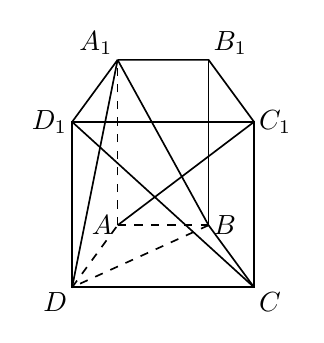
\begin{tikzpicture}[scale=1.05, semithick,
  every node/.style={inner sep=1.5pt}]
  \coordinate (D)  at (0,0);
  \coordinate (C)  at (2.2,0);
  \coordinate (A)  at (0.55,0.75);
  \coordinate (B)  at (1.65,0.75);
  \coordinate (D1) at (0,2.0);
  \coordinate (C1) at (2.2,2.0);
  \coordinate (A1) at (0.55,2.75);
  \coordinate (B1) at (1.65,2.75);

  % 被遮棱
  \draw[dashed] (D) -- (A);
  \draw[dashed] (A) -- (B);
  \draw[dashed] (A) -- (A1);
  % 题设辅助线
  \draw (D1) -- (C);
  \draw (A) -- (C1);
  \draw (A1) -- (B);
  \draw (A1) -- (D);
  \draw[dashed] (B) -- (D);
  % 可见棱
  \draw (D) -- (C) -- (C1) -- (D1) -- cycle;
  \draw (D) -- (D1);
  \draw (C) -- (C1);
  \draw (A1) -- (B1) -- (C1);
  \draw (A1) -- (D1);
  \draw (B1) -- (B);
  \draw (B) -- (C);

  % 顶点标注
  \node[below left]  at (D)  {$D$};
  \node[below right] at (C)  {$C$};
  \node[left]        at (A)  {$A$};
  \node[right]       at (B)  {$B$};
  \node[left]        at (D1) {$D_1$};
  \node[right]       at (C1) {$C_1$};
  \node[above left]  at (A1) {$A_1$};
  \node[above right] at (B1) {$B_1$};
\end{tikzpicture}
\end{center}
\nopagebreak[4]
\Needspace{4\baselineskip}
\textbf{解析}

\Needspace{5\baselineskip}
由 $AD\perp DC$、$AB\parallel DC$ 知底面 $ABCD$ 是直角梯形。设 $AD=AB=1$，则 $DC=DD_1=2$。以 $D$ 为原点，$\overrightarrow{DC}$、$\overrightarrow{DA}$、$\overrightarrow{DD_1}$ 方向分别为 $x,y,z$ 轴建立坐标系：

\nopagebreak[4]
\[D(0,0,0),\ C(2,0,0),\ A(0,1,0),\ B(1,1,0),\]

\nopagebreak[4]
\[D_1(0,0,2),\ A_1(0,1,2),\ C_1(2,0,2).\]

\Needspace{5\baselineskip}
（1）$\overrightarrow{D_1C}=(2,0,-2)$，$\overrightarrow{AC_1}=(2,-1,2)$，故

\nopagebreak[4]
\[\overrightarrow{D_1C}\cdot\overrightarrow{AC_1}=2\cdot2+0\cdot(-1)+(-2)\cdot2=0,\]

所以 $D_1C\perp AC_1$。

\Needspace{5\baselineskip}
（2）设 $E(t,0,0)$（$0\leqslant t\leqslant2$），则

\nopagebreak[4]
\[\overrightarrow{D_1E}=(t,0,-2).\]

\Needspace{5\baselineskip}
平面 $A_1BD$ 的法向量

\nopagebreak[4]
\[\boldsymbol n=\overrightarrow{DB}\times\overrightarrow{DA_1}=
\begin{vmatrix}
\boldsymbol i&\boldsymbol j&\boldsymbol k\\
1&1&0\\
0&1&2
\end{vmatrix}=(2,-2,1).\]

\Needspace{5\baselineskip}
由 $D_1E\parallel$ 平面 $A_1BD$ 得

\nopagebreak[4]
\[\overrightarrow{D_1E}\cdot\boldsymbol n=2t+0-2=0,\qquad t=1.\]

故 $E$ 为 $DC$ 的中点。此时 $D_1\notin$ 平面 $A_1BD$，线面平行成立。

（判断要点：先设出 $E$ 的坐标再用线面平行条件求参数；还要说明 $D_1$ 不在平面内，否则可能退化为线在面内。）

\gkanswer{答案：（1）证明见解析；（2）$E$ 为 $DC$ 的中点。}

\end{answer}
\begin{answer}
\gksolhead{21}{}

\textbf{题目}：

设函数 $f(x)=ax^2+b\ln x$，其中 $ab\neq0$。证明：当 $ab>0$ 时，函数 $f(x)$ 没有极值点；当 $ab<0$ 时，函数 $f(x)$ 有且只有一个极值点，并求出极值。

\Needspace{4\baselineskip}
\textbf{解析}

\Needspace{5\baselineskip}
定义域为 $(0,+\infty)$，

\nopagebreak[4]
\[f'(x)=2ax+\frac bx=\frac{2ax^2+b}{x}.\]

当 $ab>0$ 时，$a$ 与 $b$ 同号。

若 $a>0$、$b>0$，则 $2ax^2+b>0$，$f'(x)>0$；

若 $a<0$、$b<0$，则 $2ax^2+b<0$，$f'(x)<0$。

两种情形 $f'(x)$ 都不变号，故 $f(x)$ 没有极值点。

\Needspace{5\baselineskip}
当 $ab<0$ 时，$-\dfrac{b}{2a}>0$，方程 $2ax^2+b=0$ 在 $(0,+\infty)$ 内有唯一解

\nopagebreak[4]
\[x_0=\sqrt{-\frac{b}{2a}}.\]

\Needspace{5\baselineskip}
$f'(x)$ 在 $x_0$ 两侧异号，故 $x_0$ 是唯一极值点。极值为

\nopagebreak[4]
\[f(x_0)=a\left(-\frac{b}{2a}\right)+b\ln\sqrt{-\frac{b}{2a}}=-\frac b2+\frac b2\ln\left(-\frac{b}{2a}\right).\]

（判断要点：$ab>0$ 时分 $a,b$ 同正、同负两种情形，不能只讨论一种；$ab<0$ 时负号保证根号内为正。）

\gkanswer{答案：$ab>0$ 时无极值点；$ab<0$ 时有唯一极值点，极值为 $-\dfrac b2+\dfrac b2\ln\left(-\dfrac{b}{2a}\right)$。}

\end{answer}
\begin{answer}
\gksolhead{22}{}

\textbf{题目}：

已知椭圆 $C$ 的中心在坐标原点，焦点在 $x$ 轴上，椭圆 $C$ 上的点到焦点距离的最大值为 $3$，最小值为 $1$。

（1）求椭圆 $C$ 的标准方程；

（2）若直线 $l$：$y=kx+m$ 与椭圆 $C$ 相交于 $A$，$B$ 两点（$A$，$B$ 不是左右顶点），且以 $AB$ 为直径的圆过椭圆 $C$ 的右顶点。求证：直线 $l$ 过定点，并求出该定点的坐标。

\Needspace{4\baselineskip}
\textbf{解析}

\Needspace{5\baselineskip}
（1）设半长轴为 $a$、半焦距为 $c$，则 $a+c=3$、$a-c=1$，解得 $a=2$、$c=1$，$b^2=a^2-c^2=3$，故椭圆为

\nopagebreak[4]
\[\frac{x^2}{4}+\frac{y^2}{3}=1.\]

\Needspace{5\baselineskip}
（2）设 $A(x_1,y_1)$、$B(x_2,y_2)$，右顶点 $P(2,0)$。以 $AB$ 为直径的圆过 $P$ 等价于 $PA\perp PB$，即

\nopagebreak[4]
\[(x_1-2)(x_2-2)+y_1y_2=0. \tag{1}\]

\Needspace{5\baselineskip}
把 $y=kx+m$ 代入 $3x^2+4y^2=12$ 得

\nopagebreak[4]
\[(3+4k^2)x^2+8kmx+4m^2-12=0,\]

\Needspace{5\baselineskip}
故

\nopagebreak[4]
\[x_1+x_2=-\frac{8km}{3+4k^2},\qquad x_1x_2=\frac{4m^2-12}{3+4k^2}.\]

\Needspace{5\baselineskip}
又 $y_1y_2=k^2x_1x_2+km(x_1+x_2)+m^2$，代入 (1) 并通分整理得

\nopagebreak[4]
\[7m^2+16km+4k^2=0,\qquad (7m+2k)(m+2k)=0.\]

\Needspace{5\baselineskip}
若 $m=-2k$，直线 $y=k(x-2)$ 过右顶点 $P$，与 $A$、$B$ 不是左右顶点矛盾，舍去；故 $m=-\dfrac{2k}{7}$，直线为

\nopagebreak[4]
\[y=k\left(x-\frac27\right),\]

恒过定点 $\left(\dfrac27,0\right)$。

（判断要点：$m=-2k$ 是增根，必须用题设的顶点限制排除；定点可由直线方程直接读出。）

\gkanswer{答案：（1）$\dfrac{x^2}{4}+\dfrac{y^2}{3}=1$；（2）定点 $\left(\dfrac27,0\right)$。}

\end{answer}